\section{Implementation checks}\label{app:implementation}
The manual module \path{policy_adaptation/lora_training.py} implements argument validation, shared frozen base weights, Kaiming-uniform initialization of $A$, zero initialization of $B$, the scaled adapter branch, idempotent merging, nested module injection and trainable-parameter counting. The functional model check used CPU/float32 and replaced 168 projections in the 24-layer Qwen model. It reported 494,032,768 base parameters and 4,399,104 adapter parameters, or 0.8826\% of the combined model. Its forward pass and merging are functional checks, not a language-model optimizer loop.

Nine lightweight tests covered initial equality, weight sharing, a nonzero adapter formula, output-preserving and idempotent merging, frozen-base optimizer updates, nested injection/counting, invalid inputs, disjoint arithmetic data and response-only rewards with real local HTTP requests. The functional configuration used $r=8$, $\alpha=16$ and dropout 0.05; PPO used dropout 0.

\section{Search record and reproducibility boundary}\label{app:platform}
The hosted run's revised configuration started at 12:38:01 on 31 October 2026 (UTC+08:00). Its last retained event was at 13:21:18.838, and the final workspace was exported at 13:22:05. The task was then manually stopped; no automatic completion event is claimed. Five valid evaluations from seven saved proposals define the online result.

An earlier attempt produced five proposals without a valid evaluation; four completed code replies were empty. The revised run raised the output ceiling from 4,096 to 32,768 and reduced the search budget. Multiple changes and incomplete request finish reasons prevent a causal claim about which change resolved that failure. The preserved Planner records contain 70,376 tokens; this is not a complete task-cost estimate.

The source study pins LLM4AD\_Next to \code{dfde353e753e9021fffe88b5b034bf0c84d90b60}; the hosted service may use another revision. Candidate source, five evaluation records, saved configuration and independently checked geometry are published without account-specific interface captures. The actual server geometry of the online winner was not exported; the plotted winning geometry is a separate local re-execution.

\section{Historical serialization failure and successful recovery}\label{app:recovery}
An earlier FP32 T4 run completed 512 prompts / 32 rollout batches but failed at final serialization with a missing tied output-head alias:
\begin{Verbatim}[fontsize=\small,breaklines=true,frame=single]
AssertionError: mismatch keys {'base_model.model.lm_head.weight'}
RuntimeError: training failed (exit 1)
\end{Verbatim}
Its development baseline was 118/128; it has no valid final adapter or post-training validation. That baseline is not paired with the later A10 result. The preserved rounded scalar table describes that historical loop only.

\begin{center}
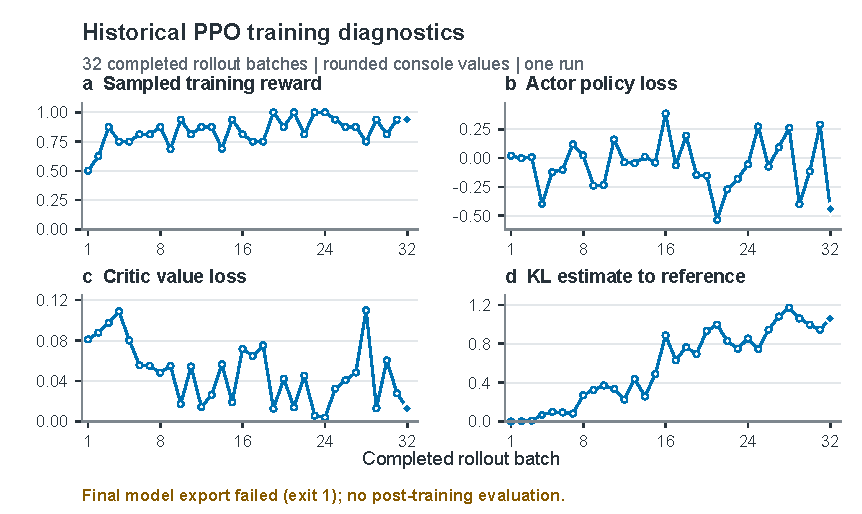
\includegraphics[width=146mm]{../../figures/observed_attempt.pdf}
\end{center}
\figcaption{fig:historical}{Historical T4 diagnostics at displayed console precision. The final-save failure occurred after these batches; the curves are neither the successful A10 run nor post-training validation.}

The save repair accepts a missing output-head name only when it aliases the exact same Parameter as the input embedding; a genuinely missing independent weight remains an error. A separate sampler repair supplies the missing \code{pad\_len=None}. The single-GPU eager route delays only unused ring-operation imports, with source hashes checked. Ring attention and packing remain disabled, and invoking that ring operation still requires FlashAttention. The declared package exception is retained: OpenRLHF 0.6.0 requires FlashAttention, which is absent. Real CUDA Actor/Critic forward/backward and FusedAdam-update checks passed before the independent 16-prompt save/reload check and fresh full run.

The successful environment used Python 3.10, PyTorch 2.5.1+cu124, Transformers 4.48.3, PEFT 0.14.0, DeepSpeed 0.16.3 and Ray 2.42.0. The evaluator may use SDPA; PPO explicitly used eager attention. The complete run finished at 09:48:14 UTC on 8 November 2026. A second invocation nine seconds later was refused by the existing-output guard. Its export manifest reports failure for that later invocation; it does not invalidate the prior successful exit, 32-batch metrics, saved finite/nonzero adapters, actual Actor reload and paired responses. Original local exports are preserved separately from the portable public evidence subset. Critic reloading and complete PPO optimizer-state recovery were not performed.

\section{Reading and reproducing the evidence}
\path{policy_adaptation/} contains the manual adapter, fixed training launcher, evaluator, reward service and compatibility repairs. Its \path{results/} records the A10 paired responses, scalar metrics and saved adapters. The historical T4 table remains separate. \path{program_search/} contains the exported best constructor, original geometry checks, saved online evaluations and independent local geometry. Plotting scripts read these saved records and do not repeat training or online search. Public copies normalize identity-bearing or machine-specific paths; this changes neither numerical results nor adapter tensors.

The fresh-environment setup recipe has not itself been validated through another complete GPU experiment. Hosted model availability, network access and GPU allocation remain external conditions. Consult the repository README for installation groups, basic checks and explicit training commands. Running a lightweight test, a plotting script or local geometry optimization is not a new PPO experiment or hosted search.
